This chapter will give a general overview on the pieces of technical equipment which we are using and show what the purpose of each one is.

\section{Prototype Hardware}

\subsection{Motors}\label{Motors}
Controlling a quadcopter can be done efficiently by using high-quality motors with fast response, which will ensure more of a stable flight. The motors must also be powerful enough to be able to lift the quadcopter and perform the required aerial movements. 

The motor that we are using is the Turnigy Multistar Brushless Motor seen in Figure \ref{motor}.

\begin{figure}[H]
  \centering
    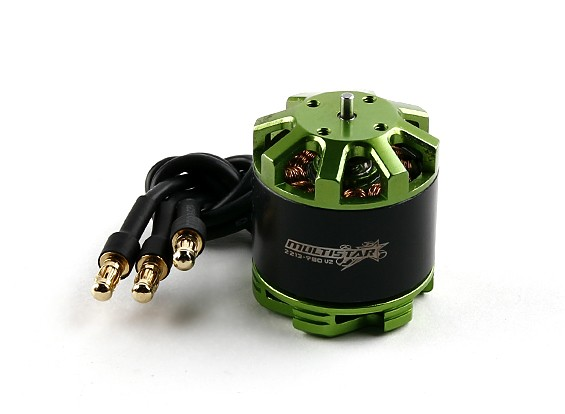
\includegraphics[width=0.5\textwidth]{images/motor.jpg}
	\caption{Turnigy Multistar 2213-980 V2 Brushless Motor.\cite{motorFigC}}
	\label{motor}
\end{figure}

\subsection{Propellers}
The propellers don't have such strict requirements as the motors. They are needed to be light and have a size and lift potential in order for the quadcopter to hover at less than 50\% of the motor capacity. For our quadcopter, we are using plasting 10x4.5'' propellers with light weight - 60g. They have a length of 254 mm and a pitch inclination of 114mm.\cite{propFig} They can be seen in Figure \ref{propeller}.

\begin{figure}[H]
  \centering
    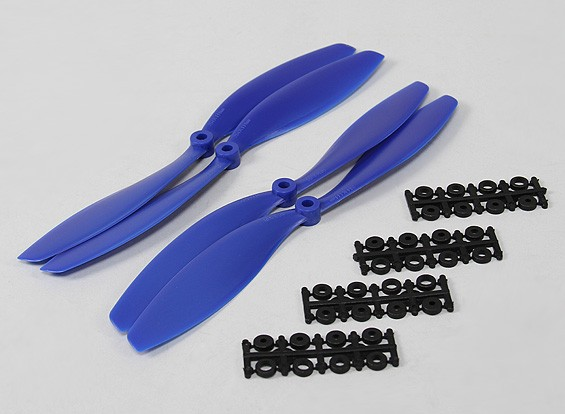
\includegraphics[width=0.5\textwidth]{images/propeller.jpg}
	\caption{Hobbyking Slowfly Propeller 10x4.5.\cite{propFig}}
	\label{propeller}
\end{figure}

\subsection{Electric Speed Controller}
Electronic Speed Controller (ESC) is a widely used device in rotorcrafts. The purpose of an ESC is to vary the electric motor's speed. They also come with programmable features, such as braking or selecting appropriate type of battery. We need the ESC to have a fast response, for the same reasons mentioned for the motors in Section \ref{Motors}. The ESC that we are using is the TURNIGY Plush 30A which is shown in Figure \ref{esc}.
 
\begin{figure}[H]
  \centering
    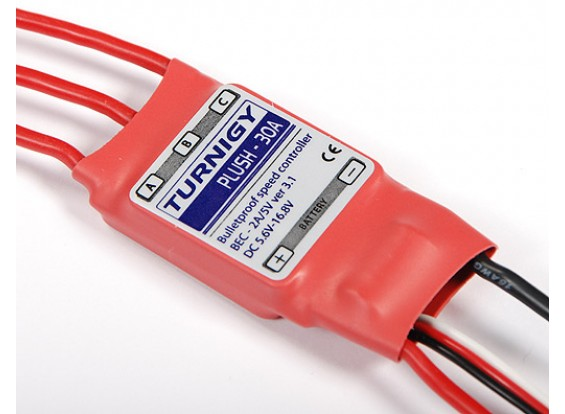
\includegraphics[width=0.5\textwidth]{images/esc.jpg}
	\caption{TURNIGY Plush 30A Speed Controller.\cite{ESCFig}}
	\label{esc}
\end{figure}

\subsection{APM Flight Controller}
ArduPilotMega (APM) is an open source unmanned aerial vehicle (UAV) platform which is able to control autonomous multicopters. It is illustrated in Figure \ref{ardupilot}. The system was improved using Inertial Measurement Unit (IMU) - a combination of accelerometer, gyroscope and a magnetometer.

\begin{figure}[H]
  \centering
    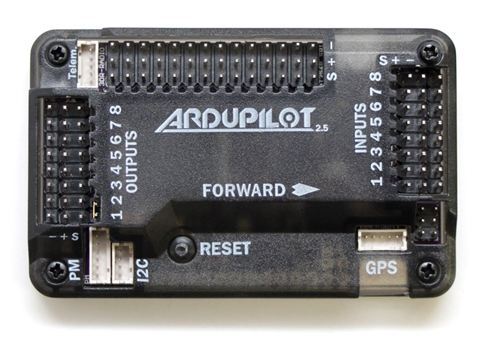
\includegraphics[width=0.5\textwidth]{images/ardupilot.jpg}
	\caption{APM 2.5 Board.\cite{APMFig}}
	\label{ardupilot}
\end{figure}

\subsection{Power Distribution Board}
To reduce the number of connections straight to the battery, we used a power distribution board made for a previous project. A board like this is an easy solution since it enables us to connect the four ESCs directly to the board and then connect the board to the battery.

\subsection{Ultrasonic Sensors}
Four HC-SR04 Ultrasonic Sensors are located on each side of the drone. Containing four pins - $V_{cc}$, $GND$, $Trig$ and $Echo$, these easy-to-use sensors detect objects at up to 400 $cm$ away.
\begin{figure}[H]
  \centering
    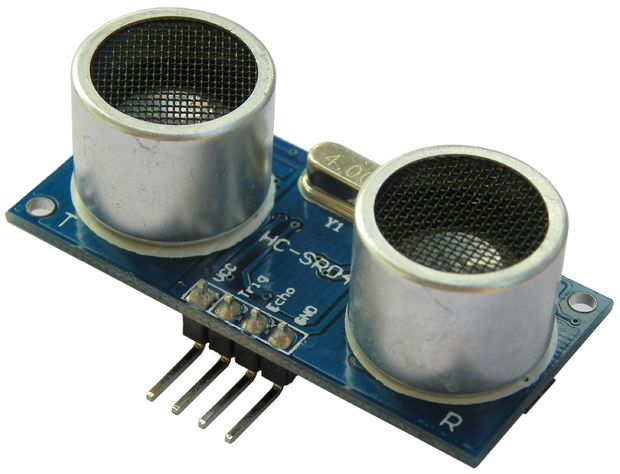
\includegraphics[width=0.4\textwidth]{images/HCSR04.jpg}
	\caption{HC-SR04 Ultrasonic Sensor.\cite{UltrasonicFig}}
	\label{HC}
\end{figure}

\subsection{Battery}
To power up our quadcopter, we will use a TURNIGY nano-tech lithium polymer battery, which can be seen in Figure \ref{battery}. Higher voltage under load, straighter discharge curves and excellent performance are the factors that make it suitable for our project. 

\begin{figure}[H]
  \centering
    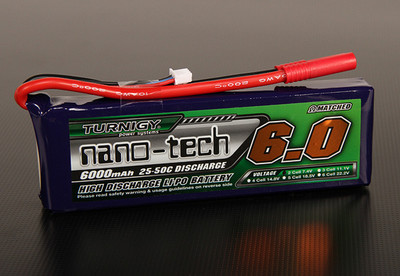
\includegraphics[width=0.5\textwidth]{images/battery.jpg}
	\caption{Turnigy Nano-tech 6000mah 3S 25~50C Lipo Pack.\cite{batteryFig}}
	\label{battery}
\end{figure}

\subsection{Drone Frame}
The drone frame, including arms for the motors, supporting legs and surface for the flight controller and battery, has been chosen and assembled by a previous group. The complete drone with all of its components put together can be seen in Figure \ref{fullDrone}.

\begin{figure}[H]
  \centering
    \includegraphics[width=0.8\textwidth]{images/fullDrone.jpg}
	\caption{Fully Assembled Drone.}
	\label{fullDrone}
\end{figure}

The wiring of the electronic components can be seen in Figure \ref{wiring}.
\begin{figure}[H]
  \centering
    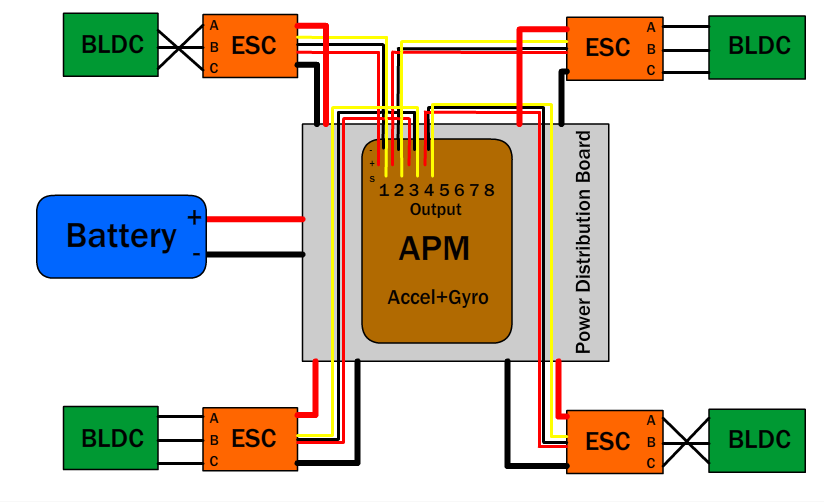
\includegraphics[width=0.8\textwidth]{images/Wiring2.png}
	\caption{Wiring of the Electronic Components.}
	\label{wiring}
\end{figure}

\section{Prototype Measurements}
The arm length has been measured to be 24.5 $cm$ and the total height of the drone has been estimated to be 13.4 $cm$.
To obtain the total weight of the drone, all parts of it, including the battery, were mounted on the frame. Then, a piece of rope was tied around all arms of the vehicle, to lift it up in the air. The other end of the rope was put on a hook of PASCO PS-3202 newtonmeter. The device was communicating its data to the PASCO Capstone software on a computer, giving a plot of force over time. The following plot can be seen in Figure \ref{weightPlot}.

\begin{figure}[H]
  \centering
    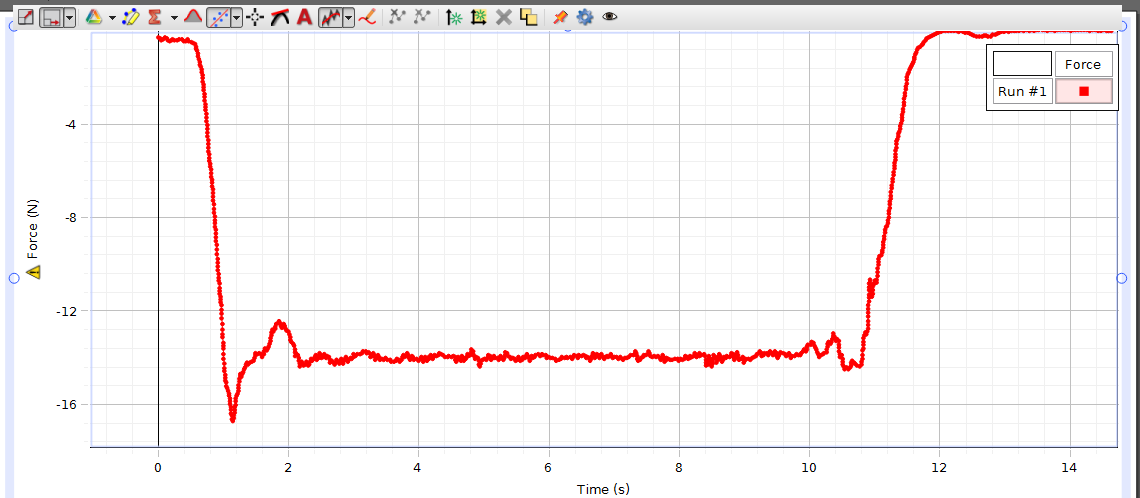
\includegraphics[width=1\textwidth]{images/weightPlot.png}
	\caption{Force vs. Time Plot of the Drone.}
	\label{weightPlot}
\end{figure}

After some time period, the prototype was lifted into the air to let the gravitational force affecting the drone be measured by the newtonmeter. It was measured that the gravitational force affecting the vehicle is approximately $14N$. From Newton's second law, we know that $F = ma$, where in this particular scenario, acceleration $a$ is equal to the gravitational force $g = 9.81m/s^2$. Therefore, the mass of the drone is equal to $m = \frac{F}{g} = \frac{14N}{9.81m/s^2} = 1.427kg$.